% fig1_system_architecture.tex — TikZ v2 optimized
% Panel (a) Device cross-section | (b) Crossbar array | (c) ViT block table
\documentclass[tikz,border=10pt]{standalone}
\usepackage{amsmath,array}
\renewcommand{\familydefault}{\sfdefault}
\usepackage{tikz}
\usetikzlibrary{positioning,arrows.meta,shapes.geometric,fit,backgrounds,calc,decorations.pathreplacing,patterns,patterns.meta}

\definecolor{anaBlue}{RGB}{80,140,210}
\definecolor{anaBlueBg}{RGB}{210,225,250}
\definecolor{digiOrange}{RGB}{220,140,60}
\definecolor{digiOrangeBg}{RGB}{255,235,210}
\definecolor{noiseRed}{RGB}{200,70,70}

\begin{document}
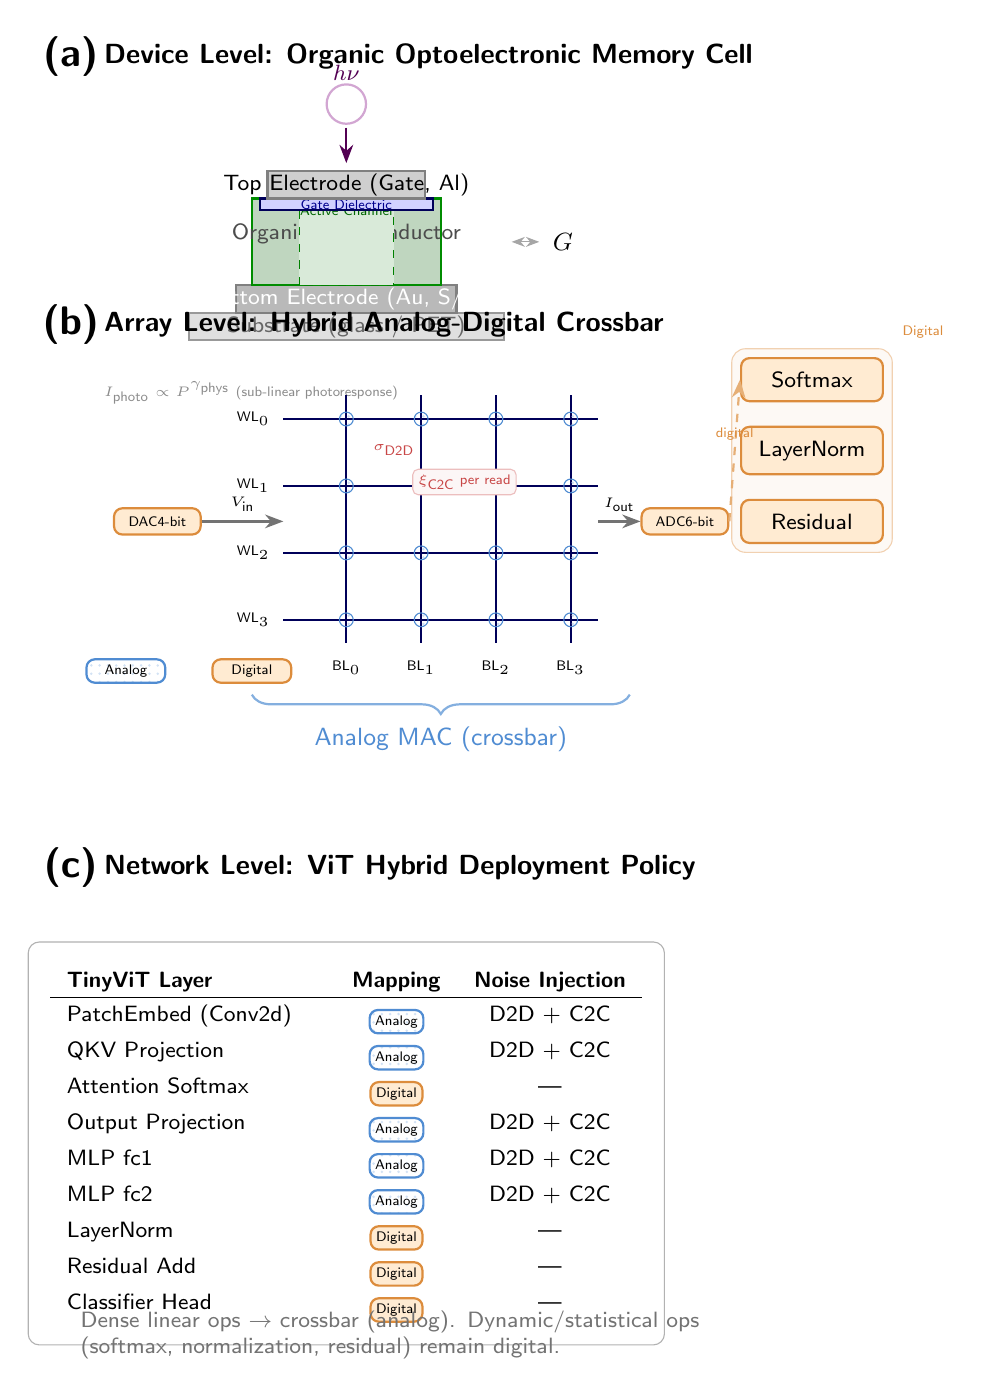
\begin{tikzpicture}[
  analogbox/.style={draw=anaBlue, fill=anaBlueBg, pattern={dots[distance=2.5pt]}, pattern color=anaBlue!25, rounded corners=3pt, thick, inner sep=5pt, font=\sffamily},
  digitalbox/.style={draw=digiOrange, fill=digiOrangeBg, rounded corners=3pt, thick, inner sep=5pt, font=\sffamily},
  boxtitle/.style={font=\bfseries\sffamily},
  panelmark/.style={font=\bfseries\sffamily\Large},
  arrowstyle/.style={->, >=Stealth, thick, draw=black!55},
]

% ===================================================================
% PANEL (a) — Device cross-section
% ===================================================================
\begin{scope}[local bounding box=panelA]
  \node[panelmark] at (-3.5, 3.6) {(a)};
  \node[boxtitle, anchor=west] at (-3.2, 3.6) {Device Level: Organic Optoelectronic Memory Cell};

  % Substrate
  \fill[black!12] (-2.0, 0) rectangle (2.0, 0.35);
  \draw[thick, black!40] (-2.0, 0) -- (2.0, 0) -- (2.0, 0.35) -- (-2.0, 0.35) -- cycle;
  \node[font=\footnotesize\sffamily, text=black!60] at (0, 0.17) {Substrate (glass / PET)};

  % Bottom electrode
  \fill[gray!55] (-1.4, 0.35) rectangle (1.4, 0.7);
  \draw[thick, black!50] (-1.4, 0.35) -- (1.4, 0.35) -- (1.4, 0.7) -- (-1.4, 0.7) -- cycle;
  \node[font=\footnotesize\sffamily, white] at (0, 0.52) {Bottom Electrode (Au, S/D)};

  % Organic semiconductor
  \fill[green!35!black!25] (-1.2, 0.7) rectangle (1.2, 1.8);
  \draw[thick, green!55!black] (-1.2, 0.7) -- (1.2, 0.7) -- (1.2, 1.8) -- (-1.2, 1.8) -- cycle;
  \node[font=\footnotesize\sffamily, text=black!70] at (0, 1.35) {Organic Semiconductor};

  % Active channel
  \fill[green!45!black!15] (-0.6, 0.7) rectangle (0.6, 1.8);
  \draw[dashed, green!50!black, thin] (-0.6, 0.7) rectangle (0.6, 1.8);
  \node[font=\tiny\sffamily, text=green!40!black] at (0, 1.65) {Active Channel};

  % Dielectric
  \fill[blue!18] (-1.1, 1.65) rectangle (1.1, 1.8);
  \draw[thick, blue!35!black] (-1.1, 1.65) -- (1.1, 1.65) -- (1.1, 1.8) -- (-1.1, 1.8) -- cycle;
  \node[font=\tiny\sffamily, text=blue!55!black] at (0, 1.72) {Gate Dielectric};

  % Top electrode
  \fill[gray!38] (-1.0, 1.8) rectangle (1.0, 2.15);
  \draw[thick, black!50] (-1.0, 1.8) -- (1.0, 1.8) -- (1.0, 2.15) -- (-1.0, 2.15) -- cycle;
  \node[font=\footnotesize\sffamily] at (0, 1.97) {Top Electrode (Gate, Al)};

  % Photon
  \draw[->, >=Stealth, thick, violet!65!black] (0, 2.7) -- (0, 2.25);
  \draw[violet!35, thick] (0, 3.0) circle (0.25);
  \node[font=\footnotesize\sffamily, violet!65!black] at (0, 3.4) {$h\nu$};

  % G label
  \draw[<->, >=Stealth, thin, black!35] (2.1, 1.25) -- (2.45, 1.25);
  \node[font=\small\sffamily, anchor=west] at (2.5, 1.25) {$G$};

  % Photo-response
  \node[font=\tiny\sffamily, text=black!45, anchor=north west] at (-3.2, -0.4)
    {$I_{\text{photo}} \propto P^{\gamma_{\text{phys}}}$ (sub-linear photoresponse)};
\end{scope}

% ===================================================================
% PANEL (b) — Crossbar array
% ===================================================================
\begin{scope}[shift={(0, -5.0)}, local bounding box=panelB]
  \node[panelmark] at (-3.5, 5.2) {(b)};
  \node[boxtitle, anchor=west] at (-3.2, 5.2) {Array Level: Hybrid Analog-Digital Crossbar};

  % Crossbar grid
  \foreach \r in {0,1,2,3} {
    \draw[thick, blue!35!black] (-0.8, 4.0-\r*0.85) -- (3.2, 4.0-\r*0.85);
    \node[font=\tiny\sffamily, anchor=east] at (-0.85, 4.0-\r*0.85) {WL$_\r$};
    \draw[thick, blue!35!black] (\r*0.95, 4.3) -- (\r*0.95, 1.15);
    \node[font=\tiny\sffamily, anchor=north] at (\r*0.95, 1.05) {BL$_\r$};
  }

  % Memory cells
  \foreach \r in {0,1,2,3} {
    \foreach \c in {0,1,2,3} {
      \node[draw=anaBlue, fill=anaBlueBg, pattern={dots[distance=1.5pt]}, pattern color=anaBlue!30, minimum size=5pt, inner sep=0pt, circle] at (\c*0.95, 4.0-\r*0.85) {};
    }
  }

  % D2D label
  \node[font=\tiny\sffamily, text=noiseRed, anchor=south west, inner sep=1pt] at (0.3, 3.5) {$\sigma_{\text{D2D}}$};

  % DAC
  \node[digitalbox, minimum width=1.1cm, font=\tiny\sffamily, inner sep=3pt] (dac) at (-2.4, 2.7) {DAC\\4-bit};
  \draw[arrowstyle] (dac.east) -- (-0.8, 2.7) node[midway, above, font=\tiny\sffamily] {$V_{\text{in}}$};

  % ADC
  \node[digitalbox, minimum width=1.1cm, font=\tiny\sffamily, inner sep=3pt] (adc) at (4.3, 2.7) {ADC\\6-bit};
  \draw[arrowstyle] (3.2, 2.7) -- (adc.west) node[midway, above, font=\tiny\sffamily] {$I_{\text{out}}$};

  % Analog bracket
  \draw[decorate, decoration={brace, mirror, amplitude=7pt}, thick, draw=anaBlue!70]
    (-1.2, 0.5) -- (3.6, 0.5) node[midway, below=8pt, font=\small\sffamily, text=anaBlue] {Analog MAC (crossbar)};

  % Digital blocks
  \node[digitalbox, minimum width=1.8cm, font=\footnotesize\sffamily, anchor=west] (softmax) at (5.0, 4.5) {Softmax};
  \node[digitalbox, minimum width=1.8cm, font=\footnotesize\sffamily, anchor=west] (ln) at (5.0, 3.6) {LayerNorm};
  \node[digitalbox, minimum width=1.8cm, font=\footnotesize\sffamily, anchor=west] (res) at (5.0, 2.7) {Residual};

  \draw[arrowstyle, draw=digiOrange!70, dashed] (adc.east) -- (softmax.west)
    node[midway, above, font=\tiny\sffamily, text=digiOrange] {digital};

  % Digital domain bg
  \begin{scope}[on background layer]
    \node[draw=digiOrange!40, rounded corners=5pt, fill=digiOrange!5, inner sep=3pt,
          fit=(softmax)(ln)(res), label={[font=\tiny\sffamily, text=digiOrange]north east:{Digital}}] {};
  \end{scope}

  % C2C label
  \node[draw=noiseRed!35, rounded corners=2pt, fill=noiseRed!5, font=\tiny\sffamily, text=noiseRed, inner sep=2pt]
    at (1.5, 3.2) {$\xi_{\text{C2C}}$ per read};

  % Legend
  \node[analogbox, minimum width=1.0cm, font=\tiny\sffamily, inner sep=2pt] at (-2.8, 0.8) {Analog};
  \node[digitalbox, minimum width=1.0cm, font=\tiny\sffamily, inner sep=2pt] at (-1.2, 0.8) {Digital};
\end{scope}

% ===================================================================
% PANEL (c) — ViT block table (tabular inside node)
% ===================================================================
\begin{scope}[shift={(0, -10.2)}, local bounding box=panelC]
  \node[panelmark] at (-3.5, 3.5) {(c)};
  \node[boxtitle, anchor=west] at (-3.2, 3.5) {Network Level: ViT Hybrid Deployment Policy};

  \node[draw=black!30, rounded corners=4pt, fill=white, inner sep=8pt] (tbl) {
    \begin{tabular}{>{\sffamily\footnotesize}p{3.2cm}>{\sffamily\footnotesize}c>{\sffamily\footnotesize}c}
      \textbf{TinyViT Layer} & \textbf{Mapping} & \textbf{Noise Injection} \\
      \hline
      PatchEmbed (Conv2d) & \tikz[baseline]\node[analogbox,inner sep=2pt,font=\tiny\sffamily]{Analog}; & D2D $+$ C2C \\
      QKV Projection & \tikz[baseline]\node[analogbox,inner sep=2pt,font=\tiny\sffamily]{Analog}; & D2D $+$ C2C \\
      Attention Softmax & \tikz[baseline]\node[digitalbox,inner sep=2pt,font=\tiny\sffamily]{Digital}; & --- \\
      Output Projection & \tikz[baseline]\node[analogbox,inner sep=2pt,font=\tiny\sffamily]{Analog}; & D2D $+$ C2C \\
      MLP fc1 & \tikz[baseline]\node[analogbox,inner sep=2pt,font=\tiny\sffamily]{Analog}; & D2D $+$ C2C \\
      MLP fc2 & \tikz[baseline]\node[analogbox,inner sep=2pt,font=\tiny\sffamily]{Analog}; & D2D $+$ C2C \\
      LayerNorm & \tikz[baseline]\node[digitalbox,inner sep=2pt,font=\tiny\sffamily]{Digital}; & --- \\
      Residual Add & \tikz[baseline]\node[digitalbox,inner sep=2pt,font=\tiny\sffamily]{Digital}; & --- \\
      Classifier Head & \tikz[baseline]\node[digitalbox,inner sep=2pt,font=\tiny\sffamily]{Digital}; & --- \\
    \end{tabular}
  };

  % Policy caption
  \node[font=\footnotesize\sffamily, text=black!55, anchor=north west, align=left, text width=8.5cm] at (-3.5, -2.0)
    {Dense linear ops $\rightarrow$ crossbar (analog).  Dynamic/statistical ops\\ (softmax, normalization, residual) remain digital.};
\end{scope}

\end{tikzpicture}
\end{document}
